\documentclass[tikz,border=5mm,12pt]{standalone}
\usepackage[fontsize=16pt]{fontsize}
\usepackage{util}
\usetikzlibrary{shapes.multipart}

\begin{document}
  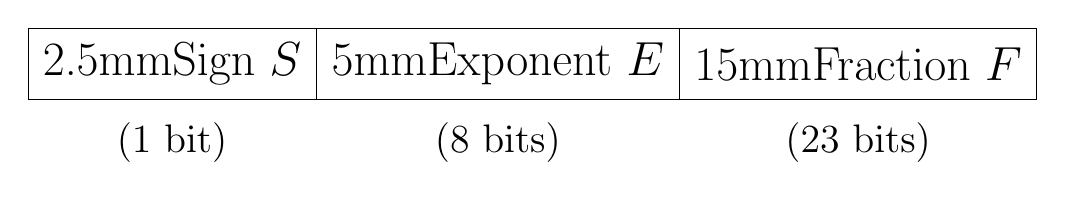
\begin{tikzpicture}[boxes/.style={draw,rectangle split,rectangle split parts=#1,anchor=center}]
    \node [name=diagram, boxes=3, rectangle split horizontal] {
      \nodepart{one} \pad{2.5mm}{Sign $S$}
      \nodepart{two} \pad{5mm}{Exponent $E$}
      \nodepart{three} \pad{15mm}{Fraction $F$}
    };

    \draw[shift=(diagram.one south)]
      node[below=1mm] {\small(1 bit)};
    \draw[shift=(diagram.two south)]
      node[below=1mm] {\small(8 bits)};
    \draw[shift=(diagram.three south)]
      node[below=1mm] {\small(23 bits)};
  \end{tikzpicture}
\end{document}
